\documentclass[11 pt]{modarticle}
\usepackage{lineno}
\usepackage{cancel}
\usepackage{tikz-cd}

% TITLE INFORMATIONS

\title{Tree-Path indices and Packness}
\date{\today}
\author[1]{$\cdot$}
%\affil[1]{}


% MATHEMATICAL OBJECTS AND NOTATIONS

\newcommand{\cN}{\mathbb{N}}
\newcommand{\cR}{\mathbb{R}}
\newcommand{\vset}{\mathcal{V}}
\newcommand{\wmap}{w}
\newcommand{\wmin}{w_m}
\newcommand{\size}[1]{|#1|}
\newcommand{\compose}{\mathbin{\circ}}

% Trees in general
\newcommand{\vsetof}[1]{V(#1)}
\newcommand{\distance}[3]{d_{#3}(#1,#2)}
\newcommand{\rtree}[2]{{#1}^{\lvert #2}}
\newcommand{\ortree}[3]{(\rtree{#1}{#2},{#3})}
\newcommand{\tclass}{\mathcal{C}}
\newcommand{\rtclass}{\mathcal{R}}

\newcommand{\smallpclass}[2]{\tclass^{#1}_{#2}}
\newcommand{\smallrpclass}[2]{\rtclass^{#1}_{#2}}
\newcommand{\greedy}[2]{\mathcal{G}(#1,#2)}

\newcommand{\pclass}[2]{\tclass^{#1}_{#2}}
\newcommand{\rpclass}[2]{\rtclass^{#1}_{#2}}

% Tree-Path indices
\newcommand{\ourproduct}{b}
\newcommand{\indexsymbol}{\mathcal{I}}
\newcommand{\tindex}[1]{\indexsymbol(#1)}
\newcommand{\rindexsymbol}{\mathcal{J}}
\newcommand{\rindex}[2]{\rindexsymbol(\rtree{#2}{#1})}
\newcommand{\aindexsymbol}{\mathcal{H}}
\newcommand{\aindex}[3]{\aindexsymbol(\rtree{#3}{#1, #2})}

% COMMENTS

\usepackage{xcolor}

\definecolor{dimmed}{gray}{0.5}
\newcommand{\old}[1]{{\color{dimmed}#1}}
\newcommand{\oldpar}[1]{{\begin{nolinenumbers}\color{dimmed}#1 \end{nolinenumbers}}}

\newcommand{\ldcomment}[1]{\textcolor{purple}{{\footnotesize Loïc:} #1}}
\newcommand{\bldcomment}[1]{\textcolor{purple}{{\footnotesize Bruno:} #1}}

\newcommand{\ldtodo}[1]{\textcolor{blue}{{\footnotesize [TODO Loïc]} #1}}
\newcommand{\ldmargin}[1]{\textcolor{blue}{*}\marginpar{\textcolor{blue}{\scriptsize Loïc: #1}}}


\begin{document}
\maketitle
\thispagestyle{empty} % removes the number of the title page

\begin{abstract}
\end{abstract}

\tableofcontents
	
\pagebreak

\section{Background}

Denote by $\cN$ the set of non-negative integers and by $\cR$ the set of real numbers. Fix some infinite set $\vset$ and some map $\wmap : \vset \to ]0,+\infty[$ that attains its minimum $\wmin > 0$ on $\vset$.

\subsection{Forests and trees, rooting and ordering}

We call forest any finite (possibly empty), simple (no loops nor multiple edges), acyclic undirected graph whose vertices belong to $\vset$. We call tree any non-empty connected forest. The set of the vertices of a tree $T$ is denoted by $\vsetof{T}$. Given vertices $u$ and $v$ of $T$ the distance $\distance{u}{v}{T}$ is the number of edges of the unique path between $u$ and $v$ in $T$.

A forest $F$ equipped with a set $R$ containing exactly one vertex from each connected component of $F$ is called a rooted forest and denoted by $\rtree{F}{R}$. %(the empty forest is rooted by $\emptyset$)
A rooted tree $\rtree{T}{\{r\}}$ is denoted by $\rtree{T}{r}$ for ease of reading. Given (possibly equal) vertices $u$ and $v$ of $T$ we say that $u$ is an ancestor of $v$ and $v$ an offspring of $u$ in $\rtree{T}{r}$ if $u$ lies on the path between $v$ and $r$ in $T$. The children of $u$ are its adjacent offspring. We call ordering of $\rtree{T}{r}$ any map $\sigma$ sending each vertex $u$ of $T$ to a total order $\sigma(u)$ on the children of $u$ in $\rtree{T}{r}$. We say that $\ortree{T}{r}{\sigma}$ is an ordered tree.

From $\ortree{T}{r}{\sigma}$ one constructs a total order on the vertices of $T$ as follows. For any two distinct vertices $u$ and $v$ of $T$ we say that $u$ is before $v$ in the \textit{BFS order} of $\ortree{T}{r}{\sigma}$ if $\distance{u}{r}{T} < \distance{v}{r}{T}$ or if $\distance{u}{r}{T} = \distance{v}{r}{T}$ and $u$ and $v$ have respective ancestors $x$ and $y$ with a common parent $z$ in $\rtree{T}{r}$ such that $x$ precedes $y$ in $\sigma(z)$. %Observe that it would imply that $v$ is not an ancestor of $u$ in $\rtree{T}{r}$.


\subsection{Isomorphism}

An isomorphism from a tree $T$ to another tree $T'$ is a bijection $f\colon \vsetof{T} \to \vsetof{T'}$ such that for every two vertices $u$ and $v$ of $T$ the edge $uv$ belongs to $T$ if and only if the edge $f(u)f(v)$ belongs to $T'$. A labeled isomorphism from $T$ to $T'$ is an isomorphism $f$ from $T$ to $T'$ such that $\wmap \compose f$ and $\wmap$ coincide on $\vsetof{T}$. A rooted isomorphism from a rooted tree $\rtree{T}{r}$ to another rooted tree $\rtree{T'}{r'}$ is an isomorphism $f$ from $T$ to $T'$ such that $f(r) = r'$. A labeled rooted isomorphism is a rooted isomorphism that is also a labeled isomorphism. An ordered isomorphism from an ordered tree $\ortree{T}{r}{\sigma}$ to another ordered tree $\ortree{T'}{r'}{\sigma'}$ is a rooted isomorphism $f$ from $\rtree{T}{r}$ to $\rtree{T'}{r'}$ such that for every two distinct children $u$ and $v$ of a vertex $w$ in $\rtree{T}{r}$ one has that $u$ is before $v$ in $\sigma(w)$ if and only if $f(u)$ is before $f(v)$ in $\sigma'(f(w))$. A labeled ordered isomorphism is an ordered isomorphism that is also a labeled isomorphism.

\subsection{Degree sequences}

The degree sequence of a tree %$T$ with $n$ vertices 
is the tuple %$(d_1, \dots, d_n)$ 
of its vertex degrees in non-increasing order. The rooted degree sequence of a rooted tree is the tuple $(d, d_1, \dots, d_{n-1})$ where $d$ is the degree of the root and $d_1, \dots, d_{n-1}$ are the degrees of the other vertices  in non-increasing order.

The \emph{BFS degree sequence} of an ordered tree is the tuple of its vertex degrees in BFS order. This sequence characterises ordered trees up to ordered isomorphism. A tuple $(d_1, \dots, d_n) \in (\cN \setminus \{0\})^n$ for some $n \geq 1$ is the BFS degree sequence of some ordered tree if and only if
\begin{equation}
	\underset{k=1}{\overset{n}{\sum}} d_k = 2n - 2 \label{eq:valid-seq}.
\end{equation}
Observe that the degree sequence of $T$ is obtained by sorting the BFS degree sequence of $\ortree{T}{r}{\sigma}$ in non-increasing order for any root $r$ and any ordering $\sigma$ of $\rtree{T}{r}$. Similarly the rooted degree sequence of $\rtree{T}{r}$ is obtained by sorting the elements of the BFS degree sequence of $\ortree{T}{r}{\sigma}$ except the first one.

In this document any BFS degree sequence, any rooted degree sequence and any degree sequence is assumed to satisfy Equation~\eqref{eq:valid-seq}.

\subsection{Classes}

\begin{defi}
For every finite non-empty $V \subset \vset$ and every non-empty set $S$ of [rooted] degree sequences of length $\size{V}$, denote by $\pclass{V}{S}$ [resp.\@ $\rpclass{V}{S}$] the set containing exactly the [rooted] trees whose vertex set is $V$ and whose [rooted] degree sequence belongs to $S$. We call [rooted] class any set of the form $\pclass{V}{S}$ [resp.\@ $\rpclass{V}{S}$].
\end{defi}

\subsection{Vertex- and edge-switches}

We now describe two operations that convert a [rooted] tree into another with the same vertices.

\begin{defi}
Assume that a tree $T$ has two distinct vertices $u$ and $v$ whose neighborhoods in $T$ are respectively $N_u$ and $N_v$. Removing the edges between $u$ and $N_u$ and between $v$ and $N_v$ and then adding the edges between $u$ and $N_v$ and between $v$ and $N_u$ gives a tree $T'$. We say that $T'$ is obtained from $T$ by the vertex-switch of the vertices $u$ and $v$. Given a vertex $r$ of $T$ we set $r' = r$ if $r \notin \{u,v\}$, $r' = v$ if $r = u$ and $r' = u$ if $r = v$ and we say that the rooted tree $\rtree{T'}{r'}$ is obtained from the rooted tree $\rtree{T}{r}$ by the rooted vertex-switch of $u$ and $v$.
\end{defi}

\bldcomment{Forgetful functor from rooted switches to switches. Works for both kinds of switch.}

\begin{tikzcd}
\rtree{T}{r} \arrow[r, ""{name=U, below}] \arrow[d]
& \rtree{T'}{r'} \arrow[d] \\
T \arrow[r, ""{name=V, above}]
& T'
\arrow[Rightarrow, from=U, to=V]
\end{tikzcd}


\begin{defi}
Assume that a tree $T$ has four pairwise-distinct vertices $x,u,v,y$ such that $xu$ and $vy$ are edges of $T$ and $u$ and $v$ both belong to the path between $x$ and $y$ in $T$. Removing the edges $xu$ and $vy$ and adding the edges $xv$ and $uy$ gives a tree $T'$. We say that $T'$ is obtained from $T$ by the edge-switch of the edges $xu$ and $yv$. Given a vertex $r$ of $T$ we say that the rooted tree $\rtree{T'}{r}$ is obtained from the rooted tree $\rtree{T}{r}$ by the rooted edge-switch of the edges $xu$ and $vy$.
\end{defi}

[Rooted] vertex- and edge-switches, collectively referred to as [rooted] switches, preserve the vertex set and the [rooted] degree sequence of a tree. Conversely, if two [rooted] trees have the same vertex set and the same [rooted] degree sequence then there is a sequence of [rooted] switches % sequence 
transforming one into the other
%some tree $T''$ whose vertex set is also $V$ and such that every vertex in $V$ has the same degree in $T'$ than in $T''$. It is known that there is an edge-switch sequence between $T'$ and $T''$ 
\cite[Theorem~4.3]{switch}. %Similarly if two rooted trees have the same vertex set and the same rooted degree sequence then there is a sequence of rooted switches transforming one into the other. 
Hence Observation~\ref{rem:proper}.

\begin{rem}\label{rem:proper}
%A class $\tclass$ is proper if and only if every tree obtained from some element of $\tclass$ by a vertex-switch or by an edge-switch also belongs to $\tclass$. A rooted class $\rtclass$ is proper if and only if every rooted tree obtained from some element of $\rtclass$ by a rooted vertex-switch or by a rooted edge-switch also belongs to $\rtclass$.
A finite, nonempty set of [rooted] trees is a [rooted] class if and only if it is closed under [rooted] switches.
\end{rem}

\bldcomment{For now we do not use arity.}
\subsection{Arity}

Consider some $k \geq 1$. We say that a tree $T$ is $k$-ary if every vertex of $T$ has degree at most $k+1$ in $T$. We say that $T$ is proper $k$-ary if every vertex of $T$ as degree either $1$ or $k+1$. We say that a rooted tree $\rtree{T}{r}$ is rooted $k$-ary if $r$ has degree at most $k$ and every (other) vertex of $T$ has degree at most $k+1$. We say that $\rtree{T}{r}$ is proper rooted $k$-ary if the degree of $r$ in $T$ is $k$ and the degree of every other vertex of $T$ is either $1$ or $k+1$. 


\section{Packed indices and majorizers}

\subsection{Greedy ordered trees}

\begin{defi}
Let $\ortree{T}{r}{\sigma}$ be an ordered tree, $v$ a vertex of $T$, some non-empty subset $S$ of the children of $v$, and some other vertex $u \neq v$ that is before $v$ in the BFS order of $\ortree{T}{r}{\sigma}$. Removing the edges between $v$ and $S$ and adding the edges between $u$ and $S$ gives a tree $T'$. We say that the tree $T'$ and the rooted tree $\rtree{T'}{r}$ are obtained from $\ortree{T}{r}{\sigma}$ by a packing.
\end{defi}

\begin{defi}
An ordered tree $\ortree{T}{r}{\sigma}$ is greedy for a [rooted] class $\tclass$ if $T$ belongs to $\tclass$, every [rooted] tree obtained from $\ortree{T}{r}{\sigma}$ by a packing does not belong to $\tclass$, and $\wmap$ is non-increasing with respect to the BFS order of $\ortree{T}{r}{\sigma}$.
\end{defi}

Consider some finite non-empty $V \subset \vset$ and some [rooted] degree sequence $D$ of length $\size{V}$. The class $\pclass{V}{\{D\}}$ [resp.\@ the rooted class $\rpclass{V}{\{D\}}$] admits, up to labeled ordered isomorphism, a unique greedy ordered tree which we denote by $\greedy{V}{D}$. The BFS degree sequence of $\greedy{V}{D}$ is $D$. Observe that $\greedy{V}{D}$ is only specified up to labeled ordered isomorphism. Given a non-empty set $S$ of [rooted] degree sequences of length $\size{V}$ the greedy ordered trees of $\pclass{V}{S}$ [resp.\@ $\rpclass{V}{S}$] all belong to $\{\greedy{V}{D'} \;:\; D' \in S\}$.

There is no clash of notation between rooted and unrooted trees since $\pclass{V}{\{D\}}$ and $\rpclass{V}{\{D\}}$ admit the same unique greedy ordered tree.
It will follow from Corollary~\ref{cor:majorization} that every class and every rooted class admits at least one greedy ordered tree.

%\begin{figure}[H]
%\small
%\centering
%\ldtodo{.}
% !!!!!!!!!!!!!!!!!!!!!! OLD AND NOT UPDATED, MAY NOT BE COHERENT ANYMORE !!!!!!!!!!!!!!!!!!
%\begin{tabular}{|c|c|c|} \hline
%	Assuming & Class of trees having $V$ as & BFS degree sequence of the \\
%	$n = \size{V}$ and... & vertex set and... & greedy ordered tree \\ \hline \hline
%	$n \geq 2$ &  & $(n-1, 1, \dots, 1)$ \\ \hline
%	$n \geq l+1$ and $l \geq 1$ & $l$ leaves & $(l, 2, \dots, 2, 1, \dots, 1)$ \\ \hline
%	$D$ is a degree sequence & degree sequence $D$ & $D$ \\ \hline
%	$n \geq 1$ and $t \in [n]$ and & degree sequence $(d_i)_{i \in [n]}$ & $(d_t, d_1, \dots, d_{t-1},d_{t+1},\dots,d_n)$ \\
%			$(d_i)_{i \in [n]}$ is a & and $r$ has degree $d_t$ & \\
%			degree sequence & & \\ \hline
%	$k \geq 1$ and $n \geq 2$ &	$k$-ary & $(\underbrace{k+1, \dots, k+1}_{p = \left\lfloor (n-2)/k \right\rfloor}, n-1-pk, 1, \dots, 1)$ \\ \hline
%	$k \geq 2$ and $l \geq 2$ & $k$-ary & $(\underbrace{k+1, \dots, k+1}_{p = \left\lfloor (l-2)/(k-1) \right\rfloor}, l-kp+p, 2,\dots,2, 1,\dots,1)$ \\
%			and $n \geq l + p + 1$ & and $l$ leaves & \\ \hline
%	$k \geq 2$ and $l \geq k+1$ & proper $k$-ary and $l$ leaves & $(k+1, \dots, k+1, 1, \dots, 1)$ \\
%			and $l \equiv 2 [k-1]$ & where $n = l + \frac{l-2}{k-1}$ & \\ \hline
%	\ldtodo{.} & rooted $k$-ary & \ldtodo{.} \\ \hline
%	\ldtodo{.} & rooted $k$-ary & \ldtodo{.} \\
%			& and $l$ leaves & \\ \hline
%	\ldtodo{.} & proper rooted $k$-ary & \ldtodo{.} \\
%			& and $l$ leaves & \\
%			& where $n=$\ldtodo{.} & \\ \hline
%\end{tabular}
%\caption{Proper classes and rooted es admitting a unique greedy ordered tree} \label{fig:greedy-elements}
%\end{figure}

\subsection{Majorizers}\label{section:majorization}

For every $n \geq 1$, every positive integer $n$-tuple $(p_1, \dots, p_n)$ and every $k \in [n]$ we introduce the notation
\begin{equation*}
	p^{\Sigma}_k = \underset{i=1}{\overset{k}{\sum}} p_i.
\end{equation*}
A positive integer tuple $(p_1, \dots, p_n)$ majorizes another positive integer tuple $(q_1, \dots, q_n)$ whenever $p^{\Sigma}_k \geq q^{\Sigma}_k$ for every $k \in [n]$. Majorization is a partial order on positive integer tuples of length $n$, including (rooted) degree sequences.% so in particular on (rooted) degree sequences of the same length.

%A degree sequence $D$ majorizes another degree sequence $E$ of the same length when $D$ majorizes $E$ as a tuple of positive integers. The same definition is taken for rooted degree sequences.

\begin{defi}
Given a [rooted] class $\pclass{V}{S}$ and some $D \in S$ we say that the tree $\greedy{V}{D}$ is a majorizer for $\pclass{V}{S}$ if $D$ is a maximal element for majorization among $S$.
\end{defi}

\begin{rem}\label{rem:majorization}
Consider some finite non-empty $V \subset \vset$ and some [rooted] degree sequence $D$ of length $\size{V}$. The [rooted] degree sequence of any [rooted] tree obtained from $\greedy{V}{D}$ by a packing is distinct from and majorizes $D$.
\end{rem}

\begin{cor}\label{cor:majorization}
Every majorizer for a [rooted] class is greedy for this same [rooted] class.
\end{cor}

\begin{prop}\label{prop:majorization}
Consider some finite non-empty $V \subset \vset$ and two [rooted] degree sequences $D$ and $D'$ of length $\size{V}$. If $D$ majorizes $D'$ and $D \neq D'$ then there is some [rooted] tree obtained from $\greedy{V}{D'}$ by a packing whose [rooted] degree sequence is majorized by $D$.
\end{prop}

\begin{proof}
We only consider the unrooted case as the rooted one is similar.

We recall that the BFS degree sequence of $\greedy{V}{D'}$ is $D'$. Let us write $D = (d_1, \dots, d_n)$ and $D' = (d'_1, \dots, d'_n)$ with $n = \size{V}$. Consider the least index $k \in [n]$ such that $d_k \neq d'_k$, which exists since $D$ and $D'$ are distinct. The difference $d_k - d'_k$ is positive since $D$ majorizes $D'$. Since both $D$ and $D'$ satisfy Equation~\eqref{eq:valid-seq} then $k < n$ and $d'_{k+1} > 1$ (we recall here that degree sequences are non-increasing tuples of positive integers). So we can consider $l > k$ maximal such that $d'_l = d'_{k+1}$ and we have $d'_l > 1$. Now let $D''$ be the $n$-tuple constructed from $D'$ by replacing the $k^{th}$ value by $d'_k+1$ and the $l^{th}$ value by $d'_l-1$. The $n$-tuple $D''$ is a non-increasing (since if $k > 1$ then $d'_k < d_k \leq d_{k-1} = d'_{k-1}$ and also since if $l < n$ then $d'_l > d'_{l+1}$) tuple of positive integers (since $d'_l > 1$) satisfying Equation~\eqref{eq:valid-seq} so $D''$ is a degree sequence. We claim that $D$ majorizes $D''$ and that $\greedy{V}{D'}$ can be packed to a tree whose degree sequence is $D''$.

Let us assume our first claim is false and obtain a contradiction. There is $i \in \{k+1, \dots, l-1\}$ such that $d^{\Sigma}_i < d''^{\Sigma}_i$. So $d^{\Sigma}_i \leq d'^{\Sigma}_i$ and we have equality since $D$ majorizes $D'$. But since $d^{\Sigma}_k > d'^{\Sigma}_k$ and since $D$ and $D'$ are non-increasing then $d_i < d'{k+1}$.  From that we conclude $d^{\Sigma}_l < (l-i) d'_{k+1} + d^{\Sigma}_i \leq (l-i) d'_{k+1} + d'^{\Sigma}_i = d'^{\Sigma}_l$ hence contradicting the assumption that $D$ majorizes $D'$. 

To prove our second claim let $u$ and $v$ denote respectively the $k^{th}$ and the $l^{th}$ vertex of $\greedy{V}{D'}$ with respect to its BFS order. Attaching one of the children of $v$ to $u$ instead of $v$ (we recall here that $d'_l > 1$ so there is such a child) gives a tree whose degree sequence is $D''$.
\end{proof}

\subsection{Packed indices}

We call [rooted] index any function mapping every [rooted] tree to a real value.

\begin{defi}\label{def:packed}
We say that an index $\phi$ is packed if whenever \textbf{A.} applies to some tree $T$ then \textbf{B.} also applies to $T$:
\begin{itemize}
	\item[\textbf{A.}] Every $T'$ obtained from $T$ by a switch satisfies $\phi(T') \leq \phi(T)$.
	\item[\textbf{B.}] There is a vertex $r$ of $T$ and an ordering $\sigma$ of $\rtree{T}{r}$ satisfying both of the following:
	\begin{itemize}
		\item[-] Every $T'$ obtained from $\ortree{T}{r}{\sigma}$ by a packing satisfies $\phi(T') > \phi(T)$.
		\item[-] The map $\wmap$ is non-increasing with respect to the BFS order of $\ortree{T}{r}{\sigma}$.
	\end{itemize}
\end{itemize}
\end{defi}

\begin{defi}
We say that a rooted index $\psi$ is packed if whenever \textbf{C.} applies to some rooted tree $\rtree{T}{r}$ then \textbf{D.} also applies to $\rtree{T}{r}$:
\begin{itemize}
	\item[\textbf{C.}] Every $\rtree{T'}{r'}$ obtained from $\rtree{T}{r}$ by a rooted switch satisfies $\psi(\rtree{T'}{r'}) \leq \psi(\rtree{T}{r})$.
	\item[\textbf{D.}] There is an ordering $\sigma$ of $\rtree{T}{r}$ satisfying both of the following:
	\begin{itemize}
		\item[-] Every $\rtree{T'}{r}$ obtained from $\ortree{T}{r}{\sigma}$ by a packing satisfies $\psi(\rtree{T'}{r}) > \psi(\rtree{T}{r})$.
		\item[-] The map $\wmap$ is non-increasing with respect to the BFS order of $\ortree{T}{r}{\sigma}$.
	\end{itemize}
\end{itemize}
\end{defi}

\begin{thm}\label{thm:maximal-is-majorizer}
Consider a class $\tclass$ and a packed index $\phi$. If a tree $T \in \tclass$ is such that $\phi(T)$ is maximal among $\tclass$ then there is a vertex $r$ of $T$ and an ordering $\sigma$ of $\rtree{T}{r}$ such that $\ortree{T}{r}{\sigma}$ is a majorizer for $\tclass$. Consider a rooted class $\rtclass$ and a packed rooted index $\psi$. If a rooted tree $\rtree{T}{r} \in \rtclass$ is such that $\psi(\rtree{T}{r})$ is maximal among $\rtclass$ then there is an ordering $\sigma$ of $\rtree{T}{r}$ such that $\ortree{T}{r}{\sigma}$ is a majorizer for $\rtclass$. 
\end{thm}

\begin{proof}
We only prove the unrooted case since the rooted case is similar. Write $\tclass = \pclass{V}{S}$ for some $V,S$. Since $\tclass$ is a class, every tree $T'$ obtained from $T$ by a switch also belongs to $\tclass$ and consequently satisfies $\phi(T') \leq \phi(T)$. But $\phi$ is packed so there is a vertex $r$ of $T$ and an ordering $\sigma$ of $\rtree{T}{r}$ satisfying two properties. First the map $\wmap$ is non-increasing with respect to the BFS order of $\ortree{T}{r}{\sigma}$. Second every $T'$ obtained from $\ortree{T}{r}{\sigma}$ by a packing satisfies $\phi(T') > \phi(T)$ and consequently does not belong to $\tclass$. So $\ortree{T}{r}{\sigma}$ is greedy for $\tclass$ and is up to labeled ordered isomorphism $\greedy{V}{D}$ for some $D \in S$. Now if $\greedy{V}{D}$ was not a majorizer for $\tclass$ then there would be a degree sequence $D' \in S$ distinct from and majorizing $D$. Proposition~\ref{prop:majorization} would then give a sequence $D_1, \dots, D_n$ of degree sequences where $n \geq 2$, $D_1 = D$, $D_n = D'$ and such that for every $k \in [n-1]$ there is some tree $T_{k+1} \in \pclass{V}{D_{k+1}}$ obtained from $\greedy{V}{D_k}$ by a packing, leading to $\phi(T_n) > \phi(T)$ since $\phi$ is packed.
\end{proof}


\begin{cor}\label{cor:maximal-finite-sum}
Theorem~\ref{thm:maximal-is-majorizer} also holds if we take $\phi$ to be a non-empty finite sum of packed indices and $\psi$ to be a non-empty finite sum of packed rooted indices.
\end{cor}

\begin{proof}
We only prove the unrooted case .  We write $\tclass = \pclass{V}{S}$ for some $V,S$. We also consider packed indices $\phi_1, \dots, \phi_n$ for some $n \geq 1$ such that $\phi = \phi_1 + \dots + \phi_n$. Let $D \in S$ being a maximal element for majorization among $S$ and $S_D \subseteq S$ be the set of degree sequences in $S$ that are majorized by $D$. Theorem~\ref{thm:maximal-is-majorizer} gives that for every $k \in [n]$ the tree underlying $\greedy{V}{D}$ is, up to labeled isomorphism, the unique element of $\smallpclass{V}{S_D}$ maximizing $\phi_k$.
\end{proof}

If $(\phi_n)_{n \in \cN}$ is a sequence of [rooted] indices, $\phi$ is a [rooted] index and $\tclass$ a [rooted] class, we say that $\phi$ is the limit of $(\phi_n)_{n \in \cN}$ on $\tclass$ when for every [rooted] tree $T \in \tclass$ the sequence $(\phi_n(T))_{n \in \cN}$ converges to $\phi(T)$.

\begin{cor}\label{cor:maximal-limit}
Consider a [rooted] class $\tclass$ and a [rooted] index $\phi$ that is, on $\tclass$, the limit of a sequence $(\phi_n)_{n \in \cN}$ of [rooted] indices where for each $n \in \cN$ the [rooted] index $\phi_n$ can be expressed as a finite sum of packed [rooted] indices. There is a majorizer $\ortree{T}{r}{\sigma}$ of $\tclass$ such that $T$ [resp.\@ $\rtree{T}{r}$] maximizes $\phi$ among $\tclass$.
\end{cor}

\begin{proof}
The result follows from Corollary~\ref{cor:maximal-finite-sum} and from the observation that $\tclass$ admits a finite number of majorizers and thus that there is an increasing map $f : \cN \to \cN$ and a majorizer $\ortree{T}{r}{\sigma}$ of $\tclass$ such that $T$ [resp.\@ $\rtree{T}{r}$] maximizes $\phi_{f(n)}$ among $\tclass$ for every $n \in \cN$.
\end{proof}

We conclude this subsection by giving two counter-examples to stronger versions of Theorem~\ref{thm:maximal-is-majorizer} and Corollaries~\ref{cor:maximal-finite-sum}~and~\ref{cor:maximal-limit}. We only deal with the unrooted case.

Let $\ortree{T_1}{r_1}{\sigma_1}$ and $\ortree{T_2}{r_2}{\sigma_2}$ be ordered trees on eight vertices with respective BFS degree sequences $(4, 2, 2, 2, 1, 1, 1, 1)$ and $(3, 3, 3, 1, 1, 1, 1, 1)$. Let $\phi_1$ be the index mapping every tree $T$ to the number of subtrees of $T$ and $\phi_2$ be the index mapping every tree $T$ to the sum over each subtree $T'$ of $T$ of $2^e$ where $e$ is the number of edges of $T'$. Both $\phi_1$ and $\phi_2$ are packed indices (as particular Tree-Path indices with $\wmap(\vset) = \{1\}$, $\lambda = 0$ and $\mu \in \{1,2\}$, see Section~\ref{section:tp-indices} for details). We have $\phi_1(T_1) = 64 > 63 = \phi_1(T_2)$ and $\phi_2(T_1) = 1042 < 1106 = \phi_2(T_2)$.

\begin{center}
	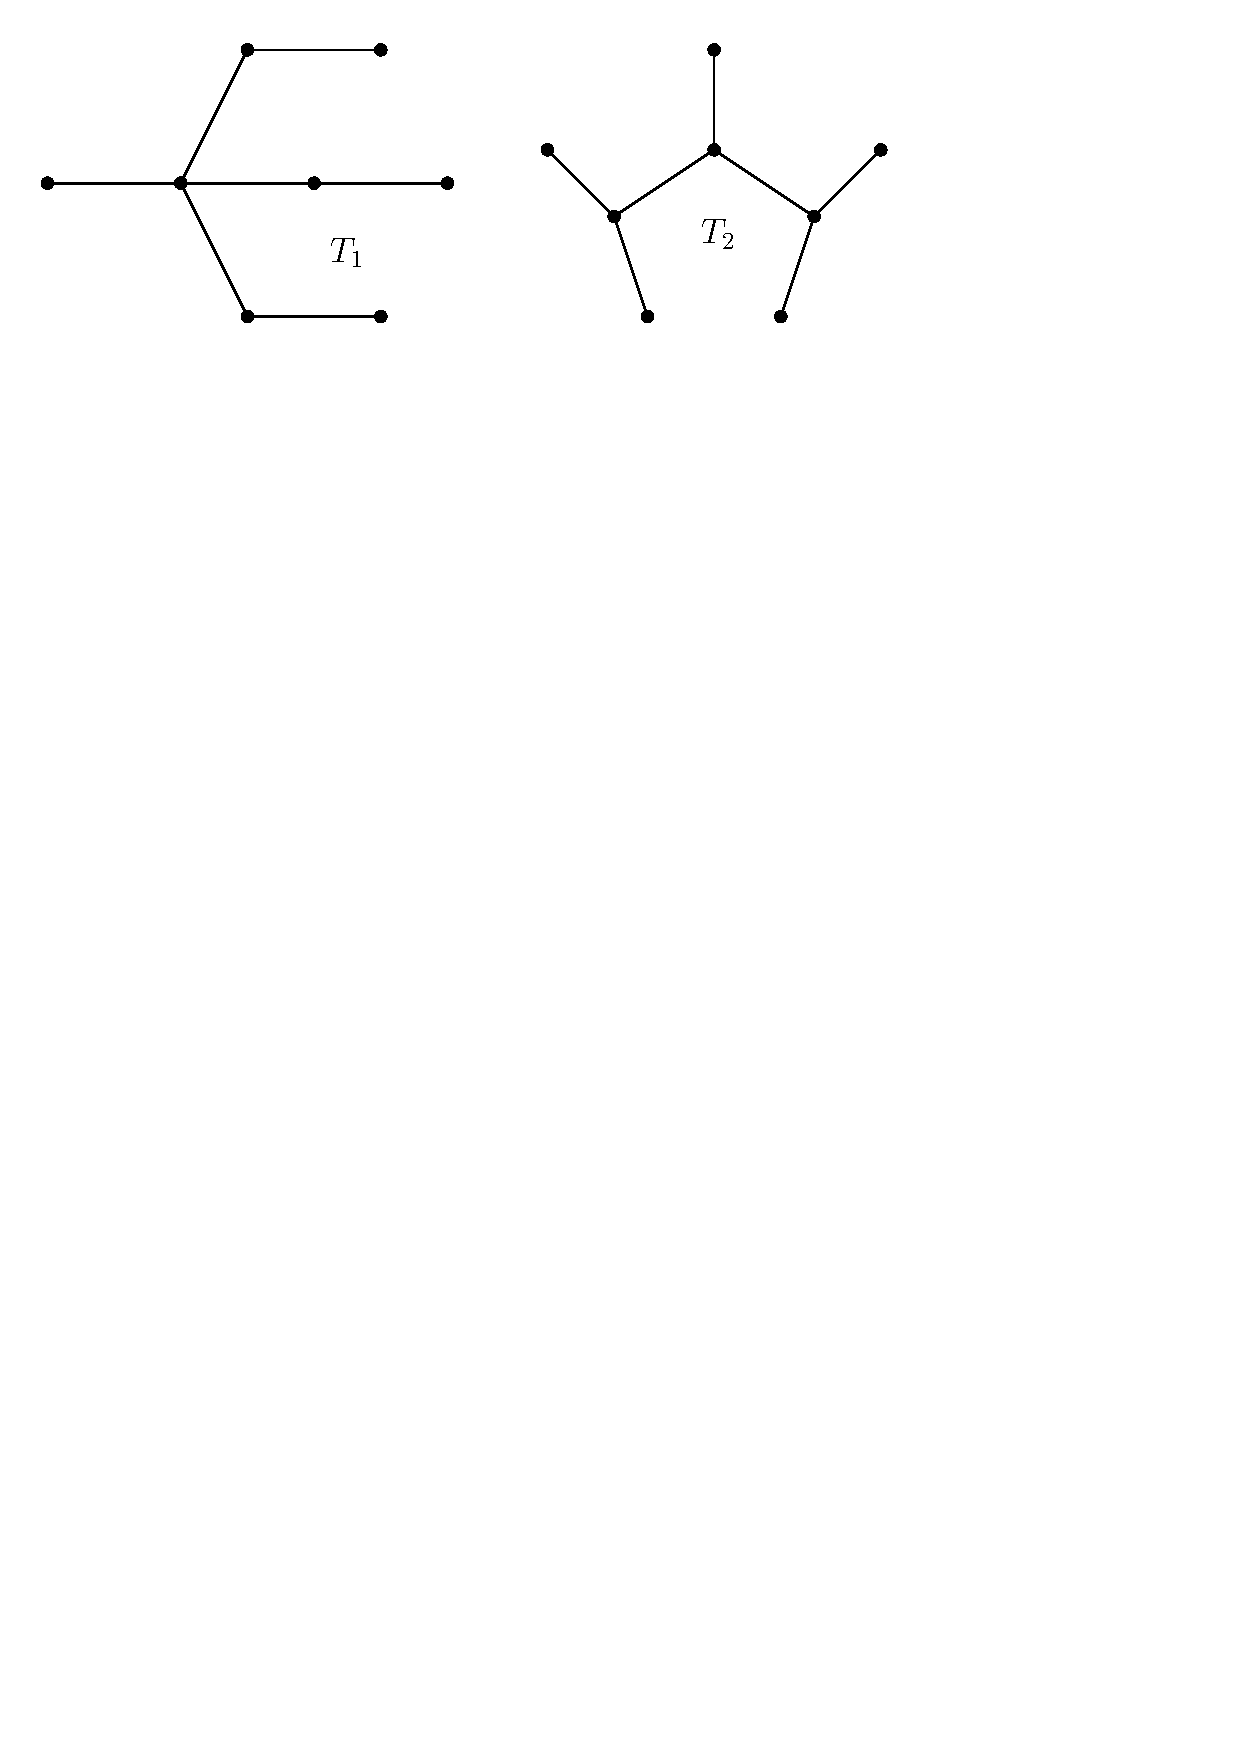
\includegraphics[scale=0.5]{figures/counter-example}
\end{center}

Finally, the index $\phi\colon T \mapsto \size{\vsetof{T}}$ is easily seen to be the limit of a sequence of packed indices from Section~\ref{section:tp-indices} (with $\wmap(\vset)= \{1\}$, $\mu = 0$ and $\lambda \rightarrow 1$), but any class with at least two trees does not admit a unique maximal element for $\phi$. 




\section{The Tree-Path indices}\label{section:tp-indices}

In this whole section we consider some $(\lambda, \mu) \in [0,+\infty)^2$.


\subsection{Introducing the Tree-Path indices}

In this subsection we define and quickly study a rooted index $\rindexsymbol$ and an index $\indexsymbol$. Both are parameterized by $\lambda, \mu$ and $\wmap$ even though this is suppressed in the notation.% in order to ease the reading.

\subsubsection{The rooted Tree-Path index}
\bldcomment{Convention: $0^0=1$, $\sum_\emptyset \dots = 0$.}

Define an internal composition law on $\cR$ by $x \star y =  x + \lambda y + \mu x y$. For convenience, we give $\star$ precedence over $+$ and $-$ and we opt for notational left-associativity, that is $x\star y \star z = (x \star y) \star z$.  It satisfies a \emph{quasi-commutative property}: 
\begin{equation}
   \text{for all $(x,y,z)\in\cR^3$,}\quad x \star y \star z = x \star z \star y.\label{eq:commutativity}
\end{equation}  
More generally, one proves by induction that, for any integer $n \geq 1$ and $(x_1,\dots,x_n)\in \cR^n$,
\[ x \star x_1 \star \dots \star x_n = x \star \left(\sum_{\substack{S \subseteq [n]\\S\neq \emptyset}} \mu^{|S|-1} \prod_{i\in S} x_i \right)
= \begin{cases} x \star \frac{ \left( \prod_{i\in [n]} (1 + \mu x_i) \right)- 1}{\mu}  & \mu \neq 0\\
x \star  \sum_{i\in [n]} x_i  & \mu = 0 \end{cases}.
\]
%It is commutative if and only if $\lambda = 1$ and associative if and only if $\lambda = 1$ or $\lambda = \mu = 0$. 




\bldcomment{$x \star y - y \star x = (x - y)(1 - \lambda)$.  Any two distinct reals commute if and only if $\lambda=1$. Associator: $x \star(y\star z) - (x\star y) \star z = z (\lambda - 1)(\lambda + \mu x)$.}

%Let $\ourproduct : \cR^2 \to \cR$ mapping every $(x,y) \in \cR^2$ to $\ourproduct(x,y) = x + \lambda y + \mu x y$. For every $(x,y,z) \in \cR^3$ the following holds:
%\begin{eqnarray}
%	\ourproduct(\ourproduct(x,y),z) = \ourproduct(\ourproduct(x,z),y). \label{eq:commutativity}
%\end{eqnarray}
%Indeed one has
%\begin{eqnarray*}
%	\ourproduct(\ourproduct(x,y),z) & = & \ourproduct(x,y) + \lambda z + \mu \ourproduct(x,y) z \\
%	& = & x + \lambda y + \mu x y + \lambda z + \mu (x + \lambda y + \mu x y) z \\
%	& = & x + (\lambda + \mu x) (y+z + \mu y z).
%\end{eqnarray*}
We define the rooted index $\rindexsymbol$ as follows. For every rooted tree $\rtree{T}{r}$ if $r$ is the only vertex of $T$ then $\rindex{r}{T} = \wmap(r)$. Otherwise $r$ has a child $u$ in $\rtree{T}{r}$ and we let $T_2$ and $T_1$ denote respectively the subtree of $T$ induced by the offspring of $u$ in $\rtree{T}{r}$ and the subtree of $T$ induced by the other vertices (that are not in the offspring). The vertices $u$ and $r$ belong respectively to $T_2$ and $T_1$ and the tree $T$ is obtained from the disjoint union of $T_2$ and $T_1$ by adding the edge $ur$. We set
\begin{eqnarray}
	\rindex{r}{T} & = & \rindex{r}{T_1} \star \rindex{u}{T_2}. \label{eq:rindex-tree-decomp}
\end{eqnarray}
Equation~\eqref{eq:commutativity} ensures that this definition does not depend on the choice of $u$. Observations~\ref{rem:rindex-minimum-value}~and~\ref{rem:rooted-examples} are straightforward.

\bldcomment{
Otherwise $r$ has some number $n$ of children $r_1,\dots,r_n$. For each $k\in[n]$ let $T_k$ be the connected component containing $r_k$ once $r$ is removed from $T$. We set
\[
\rindex{r}{T}  =  \wmap(r) \star \rindex{r_1}{T_1} \star \cdots \star \rindex{r_n}{T_n}. \label{eq:rindex-tree-fulldecomp}
\]
Equation~\eqref{eq:commutativity} ensures that this definition does not depend on the order of $r_1,\dots, r_n$.
}

\begin{rem}\label{rem:rindex-minimum-value}
The minimum of $\rindexsymbol$ is $\wmin$, which it attains on a single-vertex rooted tree. Either $\lambda + \mu > 0$ and $\rindexsymbol$ is unbounded from above, or $\lambda = \mu = 0$ and $\rindex{r}{T} = \wmap(r)$ for every rooted tree $\rtree{T}{r}$.
\end{rem}



\begin{rem}\label{rem:rooted-examples}
If $\lambda = 0$ then
\[ \rindex{r}{T} = \sum_{\substack{\text{$S$ subtree of $T$}\\r\in\vsetof{S}}} \mu^{\size{\vsetof{S}}-1} \underset{v \in \vsetof{S}}{\prod} \wmap(v).\]
If $\mu = 0$ then
\begin{eqnarray*}
	\rindex{r}{T} = \sum_{u\in \vsetof{T}} \lambda^{\distance{u}{r}{T}} \wmap(u).
\end{eqnarray*}
\end{rem}

We now extend $\rindexsymbol$ to rooted forests. For a rooted forest $\rtree{F}{R}$, letting $T_r$ be the connected component containing $r$ for each $r\in R$, set
\begin{eqnarray*}
	\rindex{R}{F} & = & \sum_{\substack{S \subseteq R\\S \neq \emptyset}} \mu^{\size{S} - 1} \underset{r \in S}{\prod} \rindex{r}{T_r}.
\end{eqnarray*}

\bldcomment{
\[ 1 + \mu \rindex{R}{F} =  \prod_{r\in R} (1 + \mu \rindex{r}{T_r})\]
}
This is consistent when $R$ is a singleton, giving $\rindex{\{r\}}{F} = \rindex{r}{T_r}$. %We define $\rindexsymbol$ to be equal to $0$ on the empty rooted forest. 
Observe also that if $\rtree{F}{R}$ is the disjoint union of $\rtree{F_1}{R_1}$ and $\rtree{F_2}{R_2}$ then
\begin{eqnarray}
	\rindex{R}{F} & = & \rindex{R_1}{F_1} + \rindex{R_2}{F_2} + \mu \rindex{R_1}{F_1} \rindex{R_2}{F_2}. \label{eq:rindex-forest-decomp}
\end{eqnarray}
We also obtain a recursion summarized by Lemma~\ref{lem:local-index-recursion}.

\begin{lem}\label{lem:local-index-recursion}
	Consider a rooted tree $\rtree{T}{r}$ and a subset $S$ of the children of $r$ in $\rtree{T}{r}$. Removing every edge $rs$ for $s \in S$ splits $T$ into a tree $T_1$ containing $r$ and a forest $F$ with $\size{S}$ components. Then
\begin{align*}
    \rindex{r}{T} &= \rindex{r}{T_1} \star \rindex{S}{F}.
	\intertext{In particular, if $S$ contains all children of $r$ then}
	\rindex{r}{T} &= \wmap(r) \star \rindex{S}{F}.
\end{align*}
\end{lem}
\bldcomment{Easy consequence of the properties of $\star$ (but those are proved similarly).}
%\begin{proof}
%We prove the result recursively on the size of $S$. The result is clear if $S$ is empty. If $S \neq \emptyset$, consider some element $u$ of $S$. Removing the edge $ur$ disconnects $T$ into two connected components, $T_r$ containing $r$ and $T_u$ containing $u$. Equation~\eqref{eq:rindex-tree-decomp} gives
%\begin{eqnarray}
%	\rindex{r}{T} = \rindex{r}{T_r} \star \rindex{u}{T_u} = \rindex{r}{T_r} + \lambda \rindex{u}{T_u} + \mu \rindex{r}{T_r} \rindex{u}{T_u}. \label{eq:local-index-recursion-1}
%\end{eqnarray}
%First assume that $S$ contains no other vertex than $u$. Then $T_u = F$ and thus Equation~\eqref{eq:rindex-forest-def} gives $\rindex{u}{T_u} = \rindex{S}{F}$. Also $r$ is the only vertex of $T_1$ so $\rindex{r}{T_1} = \wmap(r)$ holds by definition of $\rindexsymbol$ and we are done. So now assume that $S$ contains at least two vertices. 
%Applying the recursion hypothesis to $T_r$ gives
%\begin{eqnarray}
%	\rindex{r}{T_r} & = & \wmap(r) + \lambda \rindex{S'}{F'} + \mu \wmap(r) \rindex{S'}{F'} \label{eq:local-index-recursion-2}
%\end{eqnarray}
%where $S' = S \setminus \{u\}$ and $F'$ is obtained from $F$ by removing $T_u$.	Combining Equation~\eqref{eq:local-index-recursion-1} and Equation~\eqref{eq:local-index-recursion-2} gives
%\begin{eqnarray*}
%	\rindex{r}{T} & = & \wmap(r) + \lambda X + \mu \wmap(r) X = \wmap(r) \star X
%\end{eqnarray*}
%where $X = \rindex{S'}{F'} + \rindex{u}{T_u} + \mu \rindex{S'}{F'} \rindex{u}{T_u}$. We get $X = \rindex{S}{F}$ from Equation~\eqref{eq:rindex-forest-decomp}.
%\end{proof}

\subsubsection{Decomposing the rooted Tree-Path index}

We start this section with a definition that will be used in Lemma~\ref{lem:rindex-cut}. Let $T$ be a tree and $(u,v)\in\vsetof{T}^2$. Let $n=\distance{u}{v}{v} + 1$ and denote by $x_1, \dots, x_n$ the vertices of the path between $u$ and $v$ in $T$ (so $x_1 = u$ and $x_n = v$). Deleting the edges of this path disconnects $T$ into $n$ trees $(T_k)_{k\in[n]}$ with $x_k\in\vsetof{T_k}$ for each $k$. We define
\bldcomment{Poor notation}
\begin{eqnarray}
	\aindex{u}{v}{T} = \underset{k=1}{\overset{n}{\prod}} (\lambda + \mu \rindex{x_k}{T_k}). \label{eq:aindex}
\end{eqnarray}
%and observe that $\aindex{u}{v}{T} = \aindex{v}{u}{T}$.

\begin{lem}\label{lem:rindex-cut}
	Consider a tree $T_1$, vertices $u$ and $v$ in $T_1$ and a rooted forest $\rtree{F}{R}$ disjoint from $T_1$. The tree $T$ obtained from $T_1$ and $F$ by adding the edge $vr$ for every $r \in R$ has
\begin{eqnarray*}
	\rindex{u}{T} = \rindex{u}{T_1} + \aindex{u}{v}{T_1} \cdot \rindex{R}{F}.
\end{eqnarray*}
\end{lem}

\begin{proof}
This follows from Lemma~\ref{lem:local-index-recursion} by induction on $\distance{u}{v}{T_1}$.
\end{proof}

%Observe that given a tree $T$ with a vertex $u$ one has $\aindex{u}{u}{T} = \lambda + \mu \rindex{u}{T}$.

\begin{lem}\label{lem:aindex-comp}
Consider a tree $T$ with two distinct vertices $u$ and $v$ and assume $\lambda + \mu > 0$. Depending on whether $\lambda < 1$, $\lambda = 1$ or $\lambda > 1$ we have  $\aindex{u}{v}{T} < \aindex{u}{u}{T}$, $\aindex{u}{v}{T} = \aindex{u}{u}{T}$ or $\aindex{u}{v}{T} > \aindex{u}{u}{T}$ respectively.
\end{lem}

\begin{proof}
Let $n$, the path $x_1, \dots, x_n$ and the trees $(T_k)_{k\in[n]}$ be as above. Set $s_0 = 1$ and
\begin{eqnarray*}
	s_k = \aindex{u}{x_k}{T} = \underset{i=1}{\overset{k}{\prod}} (\lambda + \mu \rindex{x_i}{T_i}).
\end{eqnarray*}
The following holds recursively from Equation~\eqref{eq:rindex-tree-decomp}:
\begin{eqnarray*}
	\rindex{u}{T} = \underset{k=1}{\overset{n}{\sum}} s_{k-1} \rindex{x_k}{T_k}.
\end{eqnarray*}
Thence
\begin{eqnarray*}
	\aindex{u}{u}{T} & = & \lambda + \mu \rindex{u}{T} \\
	& = & \lambda + \underset{k=1}{\overset{n}{\sum}} s_{k-1}(\lambda + \mu \rindex{x_k}{T_k} - \lambda) \\
	& = & \lambda + \underset{k=1}{\overset{n}{\sum}} (s_k - \lambda s_{k-1}) \\
	& = & s_n + (1 - \lambda) \underset{k=1}{\overset{n-1}{\sum}} s_k.
\end{eqnarray*}
We conclude by observing that $s_1 > 0$ (since $\lambda + \mu > 0$) and $s_n = \aindex{u}{v}{T}$.
\end{proof}

\subsubsection{The Tree-Path index}

We define an index $\indexsymbol$ as follows. Consider a tree $T$. If $T$ has only one vertex $u$ then we set $\tindex{T} = \wmap(u)$. Otherwise, remove any edge $uv$ in $T$, disconnecting $T$ into two trees: let $T_1$ be the one containing $u$ and $T_2$ the one containing $v$. We recursively define $\tindex{T}$ as
\begin{eqnarray}
	\tindex{T} = \tindex{T_1} + \tindex{T_2} + (\lambda + \mu) \rindex{u}{T_1} \rindex{v}{T_2}. \label{eq:global-index-definition}
\end{eqnarray}
We will now show that this definition does not depend on the choice of $uv$.

So consider three disjoint trees $A, B$ and $X$ and assume that $A$ has a vertex $a$, that $B$ has a vertex $b$, and that $X$ has two possibly equal vertices $x$ and $y$. Let $T_{AX}$ be the tree obtained from the disjoint union of $A$ and $X$ by adding the edge $ax$. Let $T_{XB}$ be the tree obtained from the disjoint union of $B$ and $X$ by adding the edge $by$. Applying Lemma~\ref{lem:rindex-cut} gives both of the following:
\begin{eqnarray*}
	\rindex{x}{T_{XB}} & = & \rindex{x}{X} + \aindex{x}{y}{X} \rindex{b}{B}. \\
	\rindex{y}{T_{AX}} & = & \rindex{y}{X} + \aindex{x}{y}{X} \rindex{a}{A}.
\end{eqnarray*} 
Consequently
\begin{eqnarray}
	\rindex{a}{A} \rindex{x}{T_{XB}} + \rindex{b}{B} \rindex{y}{X} = \rindex{b}{B} \rindex{y}{T_{AX}} + \rindex{a}{A} \rindex{x}{X}. \label{eq:unrooted-index-consistence-claim}
\end{eqnarray}
Equation~\eqref{eq:unrooted-index-consistence-claim} proves that our definition (Equation~\eqref{eq:global-index-definition}) is consistent. Indeed let $T$ denote the tree obtained from the disjoint union of $A,B$ and $X$ by adding the two edges $ax$ and $by$. We recursively get $\tindex{A} + \tindex{T_{XB}} + (\lambda + \mu) \rindex{a}{A} \rindex{x}{T_{XB}} = \tindex{B} + \tindex{T_{AX}} + (\lambda + \mu) \rindex{b}{B} \rindex{y}{T_{AX}}$.

Remark~\ref{rem:unrooted-examples} is inferred from Remark~\ref{rem:rooted-examples} and Equation~\eqref{eq:global-index-definition}.

\begin{rem}\label{rem:unrooted-examples}
If $\lambda = 0$ then
\[ \tindex{T} = \sum_{\text{$S$ nonempty subtree of $T$}}\mu^{\size{\vsetof{S}}-1} \underset{v \in \vsetof{S}}{\prod} \wmap(v).\]
If $\mu = 0$ then 
\begin{eqnarray*}
	\tindex{T} = {\sum_{v\in\vsetof{T}} \wmap(v) } \quad + \sum_{(u,v)\in\vsetof{T}^2} \lambda^{\distance{u}{v}{T}} \wmap(u) \wmap(v).
\end{eqnarray*}
\end{rem}

Remark~\ref{rem:degenerate} is recursively inferred by Equations~\eqref{eq:rindex-tree-decomp}~and~\eqref{eq:global-index-definition}.

\begin{rem}\label{rem:degenerate}
If $\lambda = 1$ then for every tree $T$ and every vertex $r$ of $T$ we have
\begin{eqnarray*}
	\rindex{r}{T} = \tindex{T} = \sum_{\substack{S \subset \vsetof{T}\\S\neq \emptyset}} \mu^{\size{S}-1} \underset{v \in S}{\prod} \wmap(v).
\end{eqnarray*}
Observe that this quantity depends only on the set of vertices of $T$.
\end{rem}

\subsubsection{The Tree-Path index and the weights of two vertices}

\ldcomment{Can we simplify things in this section? Maybe we could merge Lemmas~\ref{lem:tindex-decomp-3}~and~\ref{lem:tindex-decomp-2}}

\begin{lem}\label{lem:tindex-decomp-1}
Let $T$ be a tree with a vertex $u$. Removing $u$ disconnects $T$ into $n$ components $T_1,\dots, T_n$ for some $n\in \cN$. For each $k\in[n]$, let $r_k$ be the neighbour of $u$ contained in $T_k$, $F_k$ be the disjoint union of $T_1, \dots, T_k$ and $R_k = \{r_1, \dots, r_k\}$. Then
\begin{eqnarray*}
	\tindex{T} & = & \wmap(u) + \left(\underset{k=1}{\overset{n}{\sum}} \tindex{T_k}\right) + (\lambda + \mu)\wmap(u)\left(\underset{k=1}{\overset{n}{\sum}}\rindex{r_k}{T_k}\right) \\
	& + & (\lambda + \mu)(\lambda + \mu \wmap(u))\left(\underset{k=1}{\overset{n-1}{\sum}}\rindex{R_k}{F_k}\rindex{r_{k+1}}{T_{k+1}}\right).
\end{eqnarray*}
\end{lem}

\begin{proof}
We prove the result by induction on $n$. If $n = 0$ then the result is clear. For $n \geq 1$, let $T'$ be the tree obtained from the disjoint union of $u$ and $F_{n-1}$ by adding the edge $u r_k$ for every $k \in [n-1]$. Applying Equation~\eqref{eq:global-index-definition} (to the edge $u r_n$) gives
\begin{eqnarray*}
	\tindex{T} & = & \tindex{T'} + \tindex{T_n} + (\lambda + \mu) \rindex{u}{T'} \rindex{r_n}{T_n}.
\end{eqnarray*}
Lemma~\ref{lem:local-index-recursion} gives $\rindex{u}{T'} = \wmap(u) + (\lambda + \mu \wmap(u)) \rindex{R_{n-1}}{F_{n-1}}$ and a recursion on $T'$ concludes.
\end{proof}

\begin{lem}\label{lem:tindex-decomp-3}
Consider two vertices $u$ and $u'$ and two rooted forests $\rtree{F}{R}$ and $\rtree{F'}{R'}$ : assume that $u$, $u'$, $F$, and $F'$ are pairwise-disjoint. Let $T$ be the tree obtained from the disjoint union of $u$, $u'$, $F$ and $F'$ by adding the edges $uu'$, $ur$ for every $r \in R$ and $u'r'$ for every $r' \in R'$ ($T$ may not contain any other vertex than $u$ and $u'$ if $F$ and $F'$ are both empty). Then
\begin{eqnarray*}
	\tindex{T} = A + B \wmap(u) + C \wmap(u') + D \wmap(u) \wmap(u')
\end{eqnarray*}
where $A,B,C$ and $D$ are independent of $\wmap(u)$ and $\wmap(u')$ and
\begin{eqnarray*}
	B & = & 1 + (\lambda + \mu)\left( \rindex{R}{F} + \lambda \rindex{R'}{F'} + \lambda \mu \rindex{R}{F} \rindex{R'}{F'} \right) \\
	C & = & 1 + (\lambda + \mu)\left( \rindex{R'}{F'} + \lambda \rindex{R}{F} + \lambda \mu \rindex{R}{F} \rindex{R'}{F'} \right) .
\end{eqnarray*}
\end{lem}

\begin{proof}
Let $T_1$ be the tree obtained from the disjoint union of $u$ and $F$ by adding the edge $ur$ for every $r \in R$. Let also $T'_1$ be the tree obtained from the disjoint union of $u'$ and $F'$ by adding the edge $u'r'$ for every $r' \in R'$. Equation~\eqref{eq:global-index-definition} (applied to the edge $uu'$) gives
\begin{eqnarray*}
	\tindex{T} = \tindex{T_1} + \tindex{T'_1} + (\lambda + \mu) \rindex{u}{T_1} \rindex{u'}{T'_1}.
\end{eqnarray*}
Lemma~\ref{lem:tindex-decomp-1} and Equation~\eqref{eq:rindex-forest-decomp} give
\begin{eqnarray*}
	\tindex{T_1} & = & E + \left(1 + (\lambda + \mu)\rindex{R}{F}\right) \wmap(u) \\
	\tindex{T'_1} & = & E' + \left(1 + (\lambda + \mu)\rindex{R'}{F'}\right) \wmap(u')
\end{eqnarray*}
where $E$ and $E'$ are independent of $\wmap(u)$ and $\wmap(u')$. Equation~\eqref{eq:rindex-forest-decomp} gives
\begin{eqnarray*}
	\rindex{u}{T_1} & = & \lambda \rindex{R}{F} + \wmap(u)(1 + \mu \rindex{R}{F}) \\
	\rindex{u'}{T'_1} & = & \lambda \rindex{R'}{F'} + \wmap(u') (1 + \mu \rindex{R'}{F'}).
\end{eqnarray*}
from which we conclude.
\end{proof}

\begin{lem}\label{lem:tindex-decomp-2}
Consider two vertices $u$ and $u'$, a tree $X$ with two possibly equal vertices $x$ and $x'$ and two (possibly empty) rooted forests $\rtree{F}{R}$ and $\rtree{F'}{R'}$ : assume that $u$, $u'$, $X$, $F$, and $F'$ are pairwise-disjoint. Let $T$ be the tree obtained from the disjoint union of $u$, $u'$, $X$, $F$ and $F'$ by adding the edges $ux$, $u'x'$, $ur$ for every $r \in R$ and $u'r'$ for every $r' \in R'$. Then
\begin{eqnarray*}
	\tindex{T} = A + B \wmap(u) + C \wmap(u') + D \wmap(u) \wmap(u')
\end{eqnarray*}
where $A,B,C$ and $D$ are independent of $\wmap(u)$ and $\wmap(u')$ and
\begin{eqnarray*}
	B & = & 1 + (\lambda + \mu) \left(\rindex{R_+}{F_+} + \lambda \aindex{x}{x'}{X} \rindex{R'}{F'} + \lambda \mu \aindex{x}{x'}{X} \rindex{R}{F} \rindex{R'}{F'}\right) \\
	C & = & 1 + (\lambda + \mu) \left(\rindex{R'_+}{F'_+} + \lambda \aindex{x}{x'}{X} \rindex{R}{F} + \lambda \mu \aindex{x}{x'}{X} \rindex{R}{F} \rindex{R'}{F'}\right) .
\end{eqnarray*}
where $F_+$ denotes the disjoint union of $F$ and $X$, $F'_+$ the disjoint union of $F'$ and $X$, $R_+ = R \cup \{x\}$ and $R'_+ = R' \cup \{x'\}$.
\end{lem}

\begin{proof}
We apply Lemma~\ref{lem:tindex-decomp-1} as follows. Here $n$ is the cardinal of $R$ plus $1$, the vertices $r_1, \dots, r_{n-1}$ are the elements of $R$ and $r_n = x$. For every $k \in [n-1]$ the tree $T_k$ is the component of $F$ containing $r_k$ and the tree $T_n$ is the tree obtained from the disjoint union of $u', X$ and $F'$ by adding the edge $u'x'$ and the edge $u' r'$ for every $r' \in R'$. Also for every $k \in [n]$ the forest $F_k$ is the disjoint union of the trees $T_1, \dots, T_k$ and $R_k = \{r_1, \dots, r_k\}$. Lemma~\ref{lem:tindex-decomp-1} gives
\begin{eqnarray}
	\tindex{T} & = & E + \tindex{T_n} + \alpha \wmap(u) + \beta \rindex{x}{T_n} + \gamma \wmap(u) \rindex{x}{T_n} \label{eq:tindex-decomp-proof-eq1}
\end{eqnarray}
where $E, \alpha, \beta$ and $\gamma$ are independent of $\wmap(u)$ and $\wmap(u')$ and
\begin{eqnarray*}
	\alpha & = & 1 + (\lambda + \mu) \left(\underset{k=1}{\overset{n-1}{\sum}} \rindex{r_k}{T_k} + \mu \underset{k=1}{\overset{n-2}{\sum}} \rindex{R_k}{F_k}\rindex{r_{k+1}}{T_{k+1}}\right) \\
	\beta & = & \lambda (\lambda + \mu)\rindex{R}{F} \\
	\gamma & = & (\lambda + \mu) (1 + \mu \rindex{R}{F}).
\end{eqnarray*}
Equation~\eqref{eq:rindex-forest-decomp} gives $\alpha = 1 + (\lambda + \mu) \rindex{R}{F}$. Lemma~\ref{lem:rindex-cut} and Equation~\eqref{eq:rindex-tree-decomp} give
\begin{eqnarray}
	\rindex{x}{T_n} = \rindex{x}{X} + \aindex{x}{x'}{X}\left(\wmap(u') + \lambda \rindex{R'}{F'} + \mu \wmap(u') \rindex{R'}{F'}\right). \label{eq:tindex-decomp-proof-eq2}
\end{eqnarray}
Now we apply Lemma~\ref{lem:tindex-decomp-1} again but this time to $T_n$. We let $p$ denote the cardinal of $R'$ plus one, $r'_1, \dots, r'_{p-1}$ denote the vertices of $R'$ and $r'_p$ denote $x'$. For every $k \in [p-1]$ the tree $T'_k$ is the component of $F'$ containing $r'_k$ and $T'_p = X$. Also for every $k \in [p]$ the forest $F'_k$ is the disjoint union of the trees $T'_1, \dots, T'_k$ and $R'_k = \{r'_1, \dots, r'_k\}$. We get
\begin{eqnarray}
	\tindex{T_n} & = & F + \Delta \wmap(u') \label{eq:tindex-decomp-proof-eq3}
\end{eqnarray}
where $F$ and $\Delta$ are independent of $\wmap(u)$ and $\wmap(u')$ and
\begin{eqnarray*}
	\Delta = 1 + (\lambda + \mu) \left(\underset{k=1}{\overset{p}{\sum}} \rindex{r'_k}{T'_k} + \mu \underset{k=1}{\overset{p-1}{\sum}} \rindex{R'_k}{F'_k} \rindex{r'_{k+1}}{T'_{k+1}}\right).
\end{eqnarray*}
Equation~\eqref{eq:rindex-forest-decomp} gives $\Delta = 1 + (\lambda + \mu) \rindex{R'_+}{F'_+}$. Combining Equations~\eqref{eq:tindex-decomp-proof-eq1}~,~\eqref{eq:tindex-decomp-proof-eq2}~and~\eqref{eq:tindex-decomp-proof-eq3} gives $\tindex{T} = A + B \wmap(u) + C \wmap(u') + D \wmap(u) \wmap(u')$ with
\begin{eqnarray*}
	B & = & \alpha + \gamma\left(\rindex{x}{X} + \lambda \aindex{x}{x'}{X} \rindex{R'}{F'}\right) \\
	C & = &  \Delta + \beta\left(\aindex{x}{x'}{X} + \mu \aindex{x}{x'}{X} \rindex{R'}{F'}\right).
\end{eqnarray*}
and we conclude by observing that Equation~\eqref{eq:rindex-forest-decomp} gives $\rindex{R}{F} + \rindex{x}{X} + \mu \rindex{R}{F} \rindex{x}{X} = \rindex{R_+}{F_+}$.
\end{proof}


\subsection{Convexity and the rooted Tree-Path index}

\begin{defi}
We say that $\rindexsymbol$ is convex if for every tree $T$ and for every three consecutive (inducing a path in this order) vertices $a,b$ and $c$ of $T$ one has
\begin{eqnarray*}
	2 \cdot \rindex{b}{T} < \rindex{a}{T} + \rindex{c}{T}.
\end{eqnarray*}
We say that $\rindexsymbol$ is concave if ${-\rindexsymbol}$ is convex. We say that $\rindexsymbol$ is degenerate if $\rindex{u}{T} = \rindex{v}{T}$ for every two vertices of every tree $T$. 
\end{defi}

\begin{prop}\label{prop:convexity}
If $\lambda + \mu \wmin \geq 1$ then, depending on whether $\lambda < 1$, $\lambda = 1$ or $\lambda > 1$ the map $\rindexsymbol$ is respectively concave, degenerate or convex. If $0 < \lambda + \mu \wmin < 1$ then $\rindexsymbol$ is neither convex, nor concave, nor degenerate.
\end{prop}

\begin{proof}
If $\lambda = 1$ we get that $\rindexsymbol$ is degenerate from Remark~\ref{rem:degenerate} %(we also obtain it from Equation~\eqref{eq:rindex-tree-decomp} and from the observation that in this particular case $\star$ commutes).
For $\lambda \neq 1$, consider a tree $T$ with three consecutive vertices $a,b$ and $c$. Removing the edges $ab$ and $bc$ splits $T$ into three components $A$, $B$ and $C$ containing $a$, $b$ and $c$ respectively. Let $x,y$ and $z$ denote respectively $\rindex{a}{A}, \rindex{b}{B}$ and $\rindex{c}{C}$. Applying Equation~\eqref{eq:rindex-tree-decomp} gives each of the following:
\begin{eqnarray*}
	\rindex{a}{T} & = & x \star (y \star z) \\
	\rindex{c}{T} & = & z \star (y \star x) \\
	\rindex{b}{T} & = & (y \star x) \star z.
\end{eqnarray*}
%Or equivalently
%\begin{eqnarray*}
%	\rindex{a}{T} & = & x + \lambda y + \lambda^2 z + \mu xy + \lambda \mu xz + \lambda \mu yz + \mu^2 xyz \\
%	\rindex{c}{T} & = & \lambda^2 x + \lambda y + z + \lambda \mu xy + \lambda \mu xz + \mu yz + \mu^2 xyz \\
%	\rindex{b}{T} & = & \lambda x + y + \lambda z + \mu xy + \lambda \mu xz + \mu yz + \mu^2 xyz.
%\end{eqnarray*}
Thence
\begin{eqnarray}
	\rindex{a}{T} + \rindex{c}{T} - 2 \rindex{b}{T} & = & x \star (y \star z) - y \star z \star x +  z \star (y \star x) - y\star x \star z \notag \\  
	& = & (x - (y\star z))(1 - \lambda) + (z - (y \star x))(1 - \lambda) \notag \\
	& = & (x + z - y - y \star (x + z)) (1 - \lambda) \notag\\
	& = & [(x + z)(1 - \lambda - \mu y) - 2y] (1 - \lambda). \label{eq:convexity}
%	\rindex{a}{T} + \rindex{c}{T} - 2 \rindex{b}{T} & = & (\lambda-1)^2 (x + z) + 2 (\lambda - 1) y + (\lambda-1) \mu y (x+z) \nonumber \\
%	& = & [\lambda - 1][(\lambda + \mu y - 1)(x+z) + 2y]. \label{eq:convexity}
\end{eqnarray}
Since $x,y,z \geq \wmin > 0$ by Remark~\ref{rem:rindex-minimum-value}, when $\lambda + \mu \wmin \geq 1$ the sign of $\rindex{a}{T} + \rindex{c}{T} - 2 \rindex{b}{T}$ is the sign of $\lambda - 1$.

On the other hand, if $0 < \lambda + \mu \wmin < 1$ we obtain that in Equation~\eqref{eq:convexity} if $y = \wmin$ and $x$ is large enough then $(\lambda + \mu y - 1)(x+z) + 2y < 0$. And if $y$ is large enough then $(\lambda + \mu y - 1)(x+z) + 2y > 0$. Both cases exist by Remark~\ref{rem:rindex-minimum-value}. Also $\lambda < 1$ holds by assumption.
\end{proof}

\subsection{Packness and the rooted Tree-Path index}

\ldtodo{I think we should be able to prove that if $\lambda + \mu > 0$ and $\lambda \neq 1$ then either $\lambda < 1$ and the rooted index $\rindexsymbol$ is packed or $\lambda > 1$ and the rooted index $-\rindexsymbol$ is packed. I think we could prove that in way similar than the way we prove packness for $\indexsymbol$ but using $\aindex{}{}{}$ instead of $\rindexsymbol$.}












\subsection{Packness and the Tree-Path index}

This section is dedicated to the proof of Theorem~\ref{thm:compacity}.

\begin{thm}\label{thm:compacity}
 Assume $\lambda + \mu \wmin \geq 1$ and $\lambda \neq 1$. If $\lambda < 1$ then $\indexsymbol$ is packed. If $\lambda > 1$ then ${-\indexsymbol}$ is packed.
\end{thm}

% \ldtodo{discuss counter-examples when $\lambda + \mu \wmin < 1$.}

We start by proving the preliminary Propositions~\ref{prop:compacity-packing}~,~\ref{prop:compacity-exchange}~and~\ref{prop:compacity-wmap}. Then we use these propositions to prove Theorem~\ref{thm:compacity}.


\begin{prop}\label{prop:compacity-packing}
Assume $\lambda + \mu > 0$ and $\lambda \neq 1$. Consider a rooted tree $\rtree{T}{r}$ with two distinct vertices $u$ and $v$ such that $v$ is not an ancestor of $u$ in $\rtree{T}{r}$. Consider also a non-empty subset $S$ of the children of $v$ in $\rtree{T}{r}$ and the tree $T'$ obtained from $T$ by disconnecting the elements of $S$ from $v$ and connecting them to $u$. If $\lambda < 1$ and $\rindex{u}{T} \geq \rindex{v}{T}$ then $\tindex{T'} > \tindex{T}$. If $\lambda > 1$ and $\rindex{u}{T} \leq \rindex{v}{T}$ then $\tindex{T'} < \tindex{T}$.
\end{prop}

\begin{proof}
We only prove the case $\lambda < 1$ and $\rindex{u}{T} \geq \rindex{v}{T}$, the other case being very similar. Let us for now assume that $S$ consists of a single vertex $s$. Removing the edge $vs$ disconnects $T$ into a tree $A$ containing $u$ and $v$, and a tree $B$ containing $s$. Equation~\eqref{eq:global-index-definition} gives
\begin{eqnarray*}
    \tindex{T'} - \tindex{T} = (\lambda + \mu) (\rindex{u}{A} - \rindex{v}{A}) \rindex{s}{B}.
\end{eqnarray*}
 Lemma~\ref{lem:rindex-cut} gives each of the following:
\begin{eqnarray*}
	\rindex{u}{T} & = & \rindex{u}{A} + \aindex{u}{v}{A} \rindex{s}{B} \\
	\rindex{v}{T} & = & \rindex{v}{A} + \aindex{v}{v}{A} \rindex{s}{B} \\
	\rindex{u}{T'} & = & \rindex{u}{A} + \aindex{u}{u}{A} \rindex{s}{B} \\
	\rindex{v}{T'} & = & \rindex{v}{A} + \aindex{u}{v}{A} \rindex{s}{B}.
\end{eqnarray*}
We assumed $\rindex{u}{T} \geq \rindex{v}{T}$ and we have $\aindex{u}{v}{A} < \aindex{u}{u}{A}$ and $\aindex{u}{v}{A} < \aindex{v}{v}{A}$ by Lemma~\ref{lem:aindex-comp} and since $\lambda < 1$. From that we deduce $\rindex{u}{A} > \rindex{v}{A}$. Finally $\tindex{T'} > \tindex{T}$ and $\rindex{u}{T'} > \rindex{v}{T'}$. The latter ensures that we can apply recursion when $S$ contains more that a single vertex.
\end{proof}

The purpose of Lemma~\ref{lem:compacity-exchange} is to ease the reading of the proof of Proposition~\ref{prop:compacity-exchange}.

\begin{lem}\label{lem:compacity-exchange}
Consider a tree $T$ with four pairwise-distinct vertices $x,u,v,y$ such that $xu$ and $yv$ are edges of $T$ and that $u$ and $v$ both belong to the path between $x$ and $y$ in $T$. Removing the edges $xu$ and $yv$ disconnects $T$ into three connected components: $T_x$ containing $x$, $T_y$ containing $y$ and $T_c$ containing $u$ and $v$. Let also $T'$ be the tree obtained from the disjoint union of $T_x, T_y$ and $T_c$ by adding the edges $xv$ and $yu$. Then
\begin{eqnarray*}
	\tindex{T'} - \tindex{T} = (\lambda + \mu) \times (\rindex{x}{T_x} - \rindex{y}{T_y}) \times (\rindex{v}{T_c} - \rindex{u}{T_c}).
\end{eqnarray*}
\end{lem}

\begin{proof}
Let $T_{cy}$ be the tree obtained from the disjoint union of $T_c$ and $T_y$ by adding the edge $vy$. Equation~\eqref{eq:global-index-definition} gives both of the following:
\begin{eqnarray*}
	\tindex{T} & = & \tindex{T_x} + \tindex{T_{cy}} + (\lambda + \mu) \rindex{x}{T_x} \rindex{u}{T_{cy}} \\
	\tindex{T_{cy}} & = & \tindex{T_c} + \tindex{T_y} + (\lambda + \mu) \rindex{v}{T_c} \rindex{y}{T_y}.
\end{eqnarray*}
Lemma~\ref{lem:rindex-cut} gives
\begin{eqnarray*}
	\rindex{u}{T_{cy}} & = & \rindex{u}{T_c} + \aindex{u}{v}{T_c} \rindex{y}{T_y}.
\end{eqnarray*}
Thence we deduce $\tindex{T} = \alpha + (\lambda + \mu) \beta$ with
\begin{eqnarray*}
	\alpha & = & \tindex{T_x} + \tindex{T_c} + \tindex{T_y} + (\lambda + \mu) \rindex{x}{T_x} \aindex{u}{v}{T_c} \rindex{y}{T_y} \\
	\beta & = & \rindex{x}{T_x}\rindex{u}{T_c} + \rindex{y}{T_y}\rindex{v}{T_c}.
\end{eqnarray*}
Applying the same arguments to $T'$ gives $\tindex{T'} = \alpha + (\lambda + \mu)\beta'$ with
\begin{eqnarray*}
	\beta' & = & \rindex{y}{T_y}\rindex{u}{T_c} + \rindex{x}{T_x}\rindex{v}{T_c}.
\end{eqnarray*}
Consequently $\tindex{T'} - \tindex{T} = (\lambda + \mu)(\beta' - \beta)$.
\end{proof}

\begin{prop}\label{prop:compacity-exchange}
Assume $\lambda + \mu > 0$ and $\lambda \neq 1$. Consider a tree $T$ with four pairwise-distinct vertices $x,u,v,y$ and assume that $xu$ and $yv$ are edges of $T$ and that $u$ and $v$ both belong to the path between $x$ and $y$ in $T$. Let $T'$ be the tree obtained from $T$ by the edge-switch of $xu$ and $yv$. Assume $\rindex{y}{T} > \rindex{x}{T}$ and $\rindex{v}{T} \leq \rindex{u}{T}$. If $\lambda < 1$ then $\tindex{T'} > \tindex{T}$. If $\lambda > 1$ then $\tindex{T'} < \tindex{T}$.
\end{prop}

\begin{proof}
We use the notations $T_x, T_y$ and $T_c$ introduced in Lemma~\ref{lem:compacity-exchange} and introduce the notations $X = \rindex{x}{T_x}, Y = \rindex{y}{T_y}, U = \rindex{u}{T_c}, V = \rindex{v}{T_c}$ and $H = \aindex{u}{v}{T}$. Equation~\eqref{eq:rindex-tree-decomp} and Lemma~\ref{lem:rindex-cut} give each of the following:
\begin{eqnarray*}
	\rindex{x}{T} & = & X + \lambda (U + HY) + \mu X (U + HY) \\
	\rindex{y}{T} & = & Y + \lambda (V + HX) + \mu Y (V + HX) \\
	\rindex{u}{T} & = & U + HY + \lambda X + \mu (U + HY) X \\
	\rindex{v}{T} & = & V + HX + \lambda Y + \mu (V + HX) Y.
\end{eqnarray*}
We assumed $\rindex{y}{T} > \rindex{x}{T}$ and $\rindex{v}{T} \leq \rindex{u}{T}$ so both of the following hold:
\begin{eqnarray*}
	0 & > & (X - Y)(1 - \lambda H) + \lambda (U - V) + \mu (UX - VY), \\
	0 & \leq & (X - Y)(\lambda - H) + (U - V) + \mu (UX - VY).
\end{eqnarray*}
To ease the reading we introduce the notations $\alpha = X - Y, \beta = U - V$ and $\gamma = UX - VY$ and write again our two equations but using this time our new notations:
\begin{eqnarray}
	0 & > & \alpha (1 - \lambda H) + \lambda \beta + \mu \gamma \label{eq:compacity-1} \\
	0 & \leq & \alpha(\lambda - H) + \beta + \mu \gamma. \label{eq:compacity-2}
\end{eqnarray}
We will now use Equation~\eqref{eq:compacity-1} and Equation~\eqref{eq:compacity-2} to prove our Proposition. Observe already that $\alpha$ and $\beta$ cannot be both equal to $0$. Indeed if $\alpha = \beta = 0$ then $\gamma = 0$ which contradicts Equation~\eqref{eq:compacity-1}.


We first assume $\lambda > 1$. We want to show $\tindex{T'} < \tindex{T}$. By Lemma~\ref{lem:compacity-exchange} it is enough to show $\alpha \beta > 0$.  Equations~\eqref{eq:compacity-1}~and~\eqref{eq:compacity-2} enforce the existence of $t \in [0,1[$ such that
\begin{eqnarray*}
	0 & = & t [\alpha (1 - \lambda H) + \lambda \beta + \mu \gamma] + (1 - t) [\alpha(\lambda - H) + \beta + \mu \gamma] \\
	& = & \alpha [(1 - \lambda H)t + (\lambda - H)(1 - t)] + \beta [\lambda t + 1 - t] \\
	& = & \alpha [\lambda - H + (1 - \lambda)t(H+1)] + \beta [(\lambda - 1) t + 1].
\end{eqnarray*}
We have $H \geq \lambda^{1 + \distance{u}{v}{T}}$ by Equation~\eqref{eq:aindex} and $\lambda > 1$ and $u \neq v$ by assumption so $H \geq \lambda^2 > \lambda$ and $\lambda - H + (1 - \lambda)t(H+1) < 0$.  Also we have $(\lambda - 1) t + 1 > 0$. That proves $\alpha \beta > 0$.

Now we assume $\lambda < 1$. We want to show $\tindex{T'} > \tindex{T}$. By Lemma~\ref{lem:compacity-exchange} it is enough to show $\alpha \beta < 0$. We will do so by case analysis : $\alpha$ is either null, negative or positive. First we assume $\alpha = 0$ and obtain a contradiction. Equations~\eqref{eq:compacity-1}~and~\eqref{eq:compacity-2} give $\beta < 0$ (since $\lambda < 1$) so $\gamma < 0$ (since $X = Y$ and $U < V$) and we contradict Equation~\eqref{eq:compacity-2}. Now we assume $\alpha < 0$ and $\beta \leq 0$ and obtain a contradiction. We have $\gamma = \alpha U + \beta Y$ so Equation~\eqref{eq:compacity-2} can be written as
\begin{eqnarray*}
	0 \leq \alpha (\lambda + \mu U - H) + \beta (1 + \mu Y).
\end{eqnarray*}
But $\lambda + \mu U = \aindex{u}{u}{T_c}$ and Lemma~\ref{lem:aindex-comp} gives $\aindex{u}{u}{T_c} > H$ (since $\lambda < 1$). So $\alpha (\lambda + \mu U - H) < 0$ and we obtain a contradiction. Finally we assume $\alpha > 0$ and $\beta \geq 0$ and obtain a contradiction. We have $\gamma = \alpha U + \beta Y$ so Equation~\eqref{eq:compacity-1} can be written as
\begin{eqnarray*}
	0 > \alpha (1 - \lambda H + \mu U) + \beta (\lambda + \mu Y)
\end{eqnarray*}
and we claim $1 - \lambda H + \mu U \geq 0$ hence obtaining a contradiction. Our claim can be obtained as follows. The assumption $\lambda < 1$ gives $1 - \lambda \geq 0 \geq (\lambda - 1) H$ and we proved $\lambda + \mu U \geq H$ previously. So $1 + \mu U \geq \lambda H$.
\end{proof}

\begin{prop}\label{prop:compacity-wmap}
Assume $\lambda + \mu > 0$. Consider a tree $T$ with two distinct vertices $u$ and $v$ and the tree $T'$ obtained from $T$ by the vertex-switch of $u$ and $v$. Assume $\rindex{u}{T} \leq \rindex{v}{T}$. If $\lambda < 1$ and $\wmap(u) > \wmap(v)$ then $\tindex{T} < \tindex{T'}$. If $\lambda > 1$ and $\wmap(u) < \wmap(v)$ then $\tindex{T} > \tindex{T'}$.
\end{prop}

\ldcomment{In the proof below do we need to distinguish whether $u$ and $v$ are adjacent or not?}

\begin{proof}
Let us first assume that $u$ and $v$ are adjacent in $T$ and prove the result in this case. Let $R$ denote the neighbors of $u$ excluding $v$ and $R'$ denote the neighbors of $v$ excluding $u$. Removing the edges between $u$ and $R$ and between $v$ and $R'$ disconnects $T$. Let $F$ be the union of the components containing an element of $R$ and $F'$ be the union of the components containing an element of $R'$. Lemma~\ref{lem:tindex-decomp-3} gives
\begin{eqnarray}
	\tindex{T} - \tindex{T'} & = & (\lambda + \mu)(\wmap(u) - \wmap(v))(1 - \lambda)(\rindex{R}{F} - \rindex{R'}{F'}). \label{eq:compacity-map-proof-eq1}
\end{eqnarray}
\bldcomment{Broken reference}
Also Equation~\eqref{eq:local-index-recursion-2} gives
\begin{eqnarray*}
	\rindex{u}{T} & = & \wmap(u) \star \rindex{R}{F} \star (\wmap(v) \star \rindex{R'}{F'}) \\
	\rindex{v}{T} & = & \wmap(v) \star \rindex{R'}{F'} \star (\wmap(u)\star \rindex{R}{F}).
\end{eqnarray*}
Observing that $ x \star y - y \star x = (1 - \lambda)(x-y)$ for every $(x, y) \in \cR^2$ we get
\begin{eqnarray}
	0 & \geq & \rindex{u}{T} - \rindex{v}{T} \nonumber \\
	& = & (1 - \lambda) \left(\wmap(u) \star \rindex{R}{F} - \wmap(v) \star \rindex{R'}{F'}\right). \label{eq:compacity-map-proof-eq2}
\end{eqnarray}
%\bldcomment{Below, case of equality to zero unaddressed.}
There are two cases. First consider $\lambda < 1$ and $\wmap(u) > \wmap(v)$.  Since both $\rindexsymbol$ and $\wmap$ are positive, %$\rindex{R}{F} \geq \rindex{R'}{F'}$ then $\wmap(u) \star \rindex{R}{F} > \wmap(v) \star \rindex{R'}{F'}$ contradicting \
Equation~\eqref{eq:compacity-map-proof-eq2} forces $\rindex{R}{F} < \rindex{R'}{F'}$ and Equation~\eqref{eq:compacity-map-proof-eq1} gives $\tindex{T} < \tindex{T'}$. Now consider $\lambda > 1$ and $\wmap(u) < \wmap(v)$. Equation~\eqref{eq:compacity-map-proof-eq2} forces $\rindex{R}{F} > \rindex{R'}{F'}$ and Equation~\eqref{eq:compacity-map-proof-eq1} gives $\tindex{T} > \tindex{T'}$.


Now we assume that $u$ and $v$ are not adjacent in $T$ and prove the result in this case. Let $x$ be the neighbor of $u$ lying on the path between $u$ and $v$ in $T$ and let $x'$ be the corresponding neighbor of $v$ ($x$ and $x'$ may be equal). Let $R_+$ denote the neighbors of $u$ and $R'_+$ the neighbors of $v$. Let also $R = R_+ \setminus \{x\}$ and $R'= R'_+ \setminus \{x'\}$. Removing the edges between $u$ and $R_+$ and between $v$ and $R'_+$ disconnects $T$. Let $X$ be the component containing $x$ and $x'$. Let $F$ be the union of the components containing an element of $R$. Let $F', F_+$ and $F'_+$ be defined similarly for $R', R_+$ and $R'_+$. We also introduce the notations $h = \aindex{x}{x'}{X}$, $j = \rindex{R}{F}$, $j_+ = \rindex{R_+}{F_+}$, $j' = \rindex{R'}{F'}$ and $j'_+ = \rindex{R'_+}{F'_+}$. Lemma~\ref{lem:tindex-decomp-2} gives
\begin{eqnarray}
	\tindex{T} - \tindex{T'} & = & (\lambda + \mu)(\wmap(u) - \wmap(v))(\alpha - \beta) \label{eq:compacity-map-proof-eq3}
\end{eqnarray}
where $\alpha = j_+ - \lambda h j$ and $\beta = j'_+ - \lambda h j'$. Equation~\eqref{eq:local-index-recursion-2} and Lemma~\ref{lem:rindex-cut} give
\begin{eqnarray*}
	\rindex{u}{T} & = & \wmap(u)\star j \star (\rindex{x}{X} + h (\wmap(v) \star j')).
\end{eqnarray*}
Observing that $x \star (y + tz) = x \star y + t (x \star z) - tx$ for every $(x,y,z,t) \in \cR^4$ we get
\begin{eqnarray*}
	\rindex{u}{T} & = & \wmap(u)\star j \star \rindex{x}{X} + h (\wmap(u)\star j \star (\wmap(v) \star j')) - h (\wmap(u) \star j) \\
	& = & \wmap(u) \star j_+ + h (\wmap(u)\star j \star (\wmap(v) \star j')) - h (\wmap(u) \star j).
\end{eqnarray*}
Similarly $\rindex{v}{T} = \wmap(v) \star  j'_+ + h \left((\wmap(v) \star j')\star (\wmap(u) \star j)\right) - h (\wmap(v) \star j')$. Now %observing that $\ourproduct(x, y) - \ourproduct(y, x) = (1 - \lambda)(x-y)$ for every $(x, y) \in \cR^2$ 
we get
\begin{eqnarray}
	0 & \geq & \rindex{u}{T} - \rindex{v}{T} \nonumber \\
	& = & \wmap(u) \star  j_+ - \wmap(v) \star j'_+ - \lambda h (\wmap(u) \star j - \wmap(v) \star j') \nonumber \\
	& = & (\wmap(u) - \wmap(v))(1 - \lambda h) + \lambda(\alpha - \beta) + \mu (\wmap(u)\alpha - \wmap(v) \beta) \nonumber \\
	& = & (\wmap(u) - \wmap(v))(1 - \lambda h + \mu \alpha)  + (\lambda + \mu \wmap(v))(\alpha - \beta). \label{eq:compacity-map-proof-eq4}
\end{eqnarray}
There are two cases. First consider $\lambda < 1$ and $\wmap(u) > \wmap(v)$. Lemma~\ref{lem:aindex-comp} gives $h \leq \lambda + \mu \rindex{x}{X}$ (with equality when $x = x'$) so $\lambda h < 1 + \mu \rindex{x}{X}$ and
\begin{eqnarray*}
	0 < (\mu j + 1)(1 + \mu \rindex{x}{X} - \lambda h) =  1 - \lambda h + \mu \alpha.
\end{eqnarray*}
So Equation~\eqref{eq:compacity-map-proof-eq4} gives $\alpha < \beta$ from which we deduce $\tindex{T} < \tindex{T'}$ by Equation~\eqref{eq:compacity-map-proof-eq4}. Now consider $\lambda > 1$ and $\wmap(u) < \wmap(v)$. Lemma~\ref{lem:aindex-comp} gives $h \geq \lambda + \mu \rindex{x}{X}$  (with equality when $x = x'$) so $\lambda h > 1 + \mu \rindex{x}{X}$ and $0 > 1 - \lambda h + \mu \alpha$. So Equation~\eqref{eq:compacity-map-proof-eq4} gives $\alpha < \beta$ from which we deduce $\tindex{T} > \tindex{T'}$ by Equation~\eqref{eq:compacity-map-proof-eq4}.
\end{proof}

We end this section with the proof of Theorem~\ref{thm:compacity}.

\begin{proof}[Proof of Theorem~\ref{thm:compacity}]
We prove only the case $\lambda < 1$, the other case being symmetric. We will show that $\indexsymbol$ is packed. Consider a tree $T$ such that every tree $T'$ obtained from $T$ by a switch satisfies $\tindex{T'} \leq \tindex{T}$. Consider some vertex $r$ of $T$ such that $\rindex{r}{T}$ is maximal among the vertices of $T$. Consider an ordering $\sigma$ of $\rtree{T}{r}$ such that in $\rtree{T}{r}$ for any two children $x$ and $y$ of a node $u$ if $x$ is before $y$ in $\sigma(u)$ then $\rindex{x}{T} \geq \rindex{y}{T}$. Our claim is that if two nodes $u$ and $v$ of $T$ are such that $u$ is before $v$ in the BFS order of $\ortree{T}{r}{\sigma}$ then $\rindex{u}{T} \geq \rindex{v}{T}$. By Propositions~\ref{prop:compacity-packing}~and~\ref{prop:compacity-wmap} our claim will prove Theorem~\ref{thm:compacity}.

So let us assume that our claim does not hold and obtain a contradiction. There are two nodes $x$ and $y$ of $T$ such that $x$ is before $y$ in the BFS order of $\ortree{T}{r}{\sigma}$ and $\rindex{x}{T} < \rindex{y}{T}$. We can assume without any loss of generality that $\distance{x}{r}{T}$ is minimal under the previous properties. If $x$ is an ancestor of $y$ then Proposition~\ref{prop:convexity} leads to a contradiction. Also $x$ and $y$ cannot have the same father in $\rtree{T}{r}$ because of our definition of $\sigma$. Hence $x$ and $y$ have distinct fathers in $\rtree{T}{r}$ that we denote by $u$ and $v$ respectively. We assumed $\rindex{x}{T} < \rindex{y}{T}$ and we have $\rindex{u}{T} \geq \rindex{v}{T}$ by minimality of $\distance{x}{r}{T}$ (since $u$ is berfore $v$ in the BFS order of $\ortree{T}{r}{\sigma}$). So by Proposition~\ref{prop:compacity-exchange} the edge-switch of $ux$ and $vy$ gives a tree $T'$ such that $\tindex{T'} > \tindex{T}$ hence contradicting our assumptions.
\end{proof}

\section{Links to the bibliography and open questions}\label{section:links}

We observe that common [rooted] indices are either cases of our [rooted] Tree-Path index with a judicious choice of parameters, or limits thereof.

\subsection{Rooted indices}

The rooted index mapping every rooted tree $\rtree{T}{r}$ to the number of subtrees of $T$ containing the root $r$ is a rooted Tree-Path index (for $\lambda = 0$, $\mu = 1$ and $\wmap(\vset) = \{1\}$). Given $\varepsilon > 0$ we denote by $\widetilde{\chi}_{\varepsilon}$ the rooted Tree-Path index given by $\lambda = 1 + \varepsilon$, $\mu = 0$ and $\wmap(\vset) = \{1\}$. The rooted index mapping every rooted tree $\rtree{T}{r}$ with $n \geq 1$ vertices to the sum over each vertex $v$ of $T$ of the distance $\distance{v}{r}{T}$ is the limit on every such $\rtree{T}{r}$ of the rooted indices
\begin{eqnarray*}
	\frac{1}{\varepsilon}(\widetilde{\chi}_{\varepsilon} - n)
\end{eqnarray*}
as $\varepsilon \rightarrow 0$.

\begin{rem}
The number of subtrees containing the root and the number of subtrees containing a given vertex are not the same thing. The first one is a rooted index. The second one is an index.
\end{rem}

\subsection{Unrooted indices}

Consider some finite $S \subset \vset$ and some $r \in \vset$. We are interested in the following indices:

\begin{align*}
    \mathbb{F}^S \colon T &\mapsto \size{\{T' \text{ subtree of } T \colon S \subseteq V(T')\}},\\
    \mathbb{F} = \mathbb{F}^{\emptyset} \colon T &\mapsto \size{\{\text{subtrees of } T\}},\\
    \mathbb{W} \colon T &\mapsto \sum_{\{u,v\} \subseteq \vsetof{T}} \distance{u}{v}{T} \quad \text{\emph{(Wiener index)}},\\
    \mathbb{W}^{\{r\}} \colon T &\mapsto \begin{cases} 0 &r \notin V(T) \\ \sum_{v \in V(T)} \distance{v}{r}{T} &r \in \vsetof{T} \end{cases},\\
    \mathbb{W}^S \colon T &\mapsto \sum_{\{u,v\} \subseteq \vsetof{T} \cap S} \distance{u}{v}{T}.
\end{align*}


%The index $\mathbb{F}^S$ maps every tree $T$ to the number of subtrees $T' \subseteq T$ such that $S \subseteq V(T')$. We write $\mathbb{F} = \mathbb{F}^{\emptyset}$ to denote the index counting the total number of subtrees. The \emph{Wiener index} $\mathbb{W}$ maps every tree $T$ to the sum over each unordered pair $\{u,v\} \subseteq V(T)$, of the distance $\distance{u}{v}{T}$ between $u$ and $v$ in $T$. The index $\mathbb{W}^{\{r\}}$ maps $T$ to $0$ if $r \notin V(T)$. Otherwise $\mathbb{W}^{\{r\}}(T)$ is the sum over every $v \in V(T)$ of the distance $\distance{v}{r}{T}$ between $v$ and $r$ in $T$. If $\size{S} \geq 2$ then the index $\mathbb{W}^S$ maps $T$ to the sum over each unordered pair $\{u, v\} \subseteq V(T) \cap S$, $u \neq v$, of the distance $\distance{u}{v}{T}$ between $u$ and $v$ in $T$.

Given $X \subseteq \vset$, $\rho \geq 1$ and $\lambda, \mu \geq 0$, we set for every $v \in \vset$ the value $\wmap(v)$ to $\rho$ if $v \in X$ or $1$ if $v \notin X$ and we define $\chi^{\lambda, \mu}_{X, \rho}$ as the Tree-Path index corresponding to $\lambda, \mu$ and $w$. We also consider a class $\tclass$ and let $V$ denote the vertex set of the trees in $\tclass$.


We have $\mathbb{F} = \chi^{0,1}_{\emptyset, 1}$, a packed index, whereas $\mathbb{F}^S$ is a limit of packed indices:
\begin{eqnarray*}
	\mathbb{F}^S = \lim_{\rho\to +\infty} \frac{1}{\rho^{\size{S}}} \chi^{0,1}_{S,\rho} \quad \text{on all trees.}
\end{eqnarray*}
\bldcomment{Below, $\epsilon^2 \rho = 1$ should work(?). I find
\[ \rho^{-3/2}\chi^{1 + \rho^{-1/2},0}_{S,\rho} - \rho^{1/2} \binom{\size{S \cap V}}{2} \to \mathbb{W}^S\]}

If $\size{S} \geq 2$ then $-\mathbb{W}^S$ is a limit of packed indices:
\begin{eqnarray*}
	\mathbb{W}^S = \lim_{\varepsilon \to 0} \lim_{\rho\to +\infty} \frac{1}{\varepsilon}\left(\frac{1}{\rho^2} \chi^{1+\varepsilon,0}_{S,\rho} - {\binom{\size{S \cap V}}{2}} \right) \quad \text{on $\tclass$.}
\end{eqnarray*}
\bldcomment{Below: should it not be $\lim_{\epsilon \to 0} \lim_{\rho\to\infty}\frac{1}{\varepsilon}\left(\frac{1}{\rho}\chi^{1+\varepsilon,0}_{\{r\},\rho}-\size{V} - 1\right)$? Also $\epsilon \rho = 1$ seems fine, that is
\[
	\mathbb{W}^{\{r\}} = \lim_{\rho\to\infty}\chi^{1+\rho^{-1},0}_{\{r\},\rho}- \rho \left(\size{V} + 1\right) \quad \text{on $\tclass$}.
\]}
Finally if $r \in V$ then $-\mathbb{W}^{\{r\}}$ is a limit of packed indices:
\begin{eqnarray*}
	\mathbb{W}^{\{r\}} = \lim_{\epsilon \to 0} \lim_{\rho\to\infty}\frac{1}{\varepsilon}\left(\frac{1}{\rho}\chi^{1+\varepsilon,0}_{\{r\},\rho}-\size{V}\right) \quad \text{on $\tclass$}.
\end{eqnarray*}
\subsection{Some open questions}

Some open questions:
\begin{itemize}
\item[\textbf{Q1.}] Is the (unrooted) Tree-Path index packed (at least in some cases) when $0 < \lambda + \mu \wmin < 1$?
\item[\textbf{Q2.}] In Observations~\ref{rem:rooted-examples}~,~\ref{rem:unrooted-examples}~and~\ref{rem:degenerate} we obtained "explicit" formulas for both the rooted and the unrooted Tree-Path index for particular values of $\lambda$ and $\mu$. Is there such a formula in general? Or at least for other values of $\lambda$ and $\mu$?
\item[\textbf{Q3.}] Are there other indices that are packed? (Probably the opposite of the sum of the distances to the root and the opposite of the Wiener index if I remember correctly, but here we only proved that they are limits of packed indices) Could we derive some simple conditions for an index to be packed?
\item[\textbf{Q4.}] Can the notion of packness be extended to encode the optimal trees for the Hosoya and the Merrifield–Simmons\cite{andriantiana} indices?
\end{itemize}

\bldcomment{As for Q2, the rooted Tree-Path index can be seen as a formal polynomial on the vertices (evaluated by replacing each vertex with its value under $\wmap$). It seems possible to describe the coefficient corresponding to a given subset of vertices. For example, for a path of length $k$ from the root the coefficient will be $\mu^{k-1}$. For such a path minus $t$ vertices we will have $\lambda^t\mu^{k-t-1}$, etc.}

\pagebreak
\addcontentsline{toc}{section}{References}
\bibliographystyle{alphaurl}
\bibliography{biblio}



\pagebreak
\appendix


\end{document}

